% Edit this section directly. Styling is in raylo-report.sty.
\section{The machine-learning tier: transformer models}
The linear classifier has one structural weakness. It memorises the character patterns of merchants it has seen and has no way to generalise to a merchant it has not. Frontier language models read unseen merchants at 84\% against the linear model's 54\% on the same holdout, but cannot run at decision time. The question for September was whether a small transformer, trained to run on CPU, could carry some of that reading ability into the pipeline.

\subsection{What a transformer is, in plain terms}
A transformer is a type of neural network built for sequences: words in a sentence, or here, the pieces of a bank narrative. Older text models read left to right and carried a fading memory. A transformer instead lets every piece of the input look at every other piece at once and decide how much attention to pay to each. Reading \emph{SKYBET 04321 LEEDS}, the model learns that \emph{SKYBET} is the piece that matters and that \emph{04321} and \emph{LEEDS} are a till number and a town that appear after many merchants and carry little meaning. That mechanism, called attention, is what lets the model generalise to a merchant it has never seen: it has learned which parts of a narrative tend to name the business and which are noise.

The model learns in two stages. First it is \emph{pretrained} on a very large pile of unlabelled text with a fill-in-the-blank exercise: a word is hidden and the model must guess it from the words around it. Doing this millions of times teaches it the language of the domain with no human labels at all. Then it is \emph{fine-tuned} on a much smaller set of labelled examples for the actual task, here the 275 categories. Because the pretraining already taught it what bank narratives look like, the fine-tuning needs far fewer labels than training from scratch would.

There are two families. \emph{Generative} transformers, such as the large language models used for labelling, write text out one word at a time. \emph{Encoder} transformers read text in and produce a compact numerical summary of it, a vector, which a small final layer turns into a decision. Our task is a choice from a closed list, so an encoder is the natural fit: smaller, faster, deterministic, and it cannot invent a category that does not exist.

\subsection{How our model reads a transaction}
Figure 6a follows one transaction through the model. The raw Plaid row is rewritten as a short sentence that carries everything the model is allowed to see: the direction, a coarse amount band, the merchant string and the bank narrative. That sentence is split into word-pieces, including 4,000 pieces added specifically for this domain (bank abbreviations, retailer stems, benefit codes), and each piece becomes a number. Six layers of attention then refine those numbers so that each piece is understood in the context of the others. The pieces are averaged into one 768-number summary of the transaction. Two small final layers read that summary: one scores all 275 leaves, the other all 29 general categories, and a consistency term during training keeps the two in agreement. Last, a direction mask sets to zero any category that cannot occur for that direction, so a debit can never be labelled salary. The highest remaining score is the answer, and its margin over the runner-up is the model's confidence.

\begin{figure}[H]
\centering
\ChartTitle{Figure 6a. One transaction through the categorisation transformer}
\resizebox{\linewidth}{!}{%
\begin{tikzpicture}[
  x=1mm,y=1mm,font=\footnotesize,
  box/.style={draw=Blue,fill=BlueTint,rounded corners=1.2mm,line width=0.4pt,align=center,inner sep=2.2mm,text width=30mm},
  data/.style={draw=Muted,fill=white,rounded corners=1.2mm,line width=0.4pt,align=left,inner sep=2.2mm,text width=36mm},
  result/.style={draw=Blue,fill=Blue,text=white,rounded corners=1.2mm,line width=0.4pt,align=center,inner sep=2.2mm,text width=30mm},
  lab/.style={font=\scriptsize\color{Muted},align=center},
  arr/.style={-{Stealth[length=2mm]},line width=0.5pt,color=Muted}]
  \node[data] (raw) at (0,0) {\textbf{Raw Plaid row}\\merchant: Sky Bet\\description: SKYBET 04321 LEEDS\\amount: 20.00, direction: debit};
  \node[data,text width=36mm] (sent) at (0,-24) {\textbf{One sentence}\\{\ttfamily [DEBIT] [AMT 10--50]}\\{\ttfamily sky bet | skybet 04321 leeds}};
  \node[data,text width=36mm] (tok) at (0,-46) {\textbf{Word-pieces}\\{\ttfamily debit · amt · sky · bet · sky · bet · 04321 · leeds}\\30,000 standard + 4,000 domain pieces};
  \node[box,text width=40mm,minimum height=52mm] (enc) at (62,-23) {\textbf{Encoder}\\DistilBERT, 6 layers, 66M parameters\\[3pt]Every piece attends to every other piece; \emph{skybet} is weighed up, \emph{04321} and \emph{leeds} weighed down\\[3pt]Pretrained on 21.5M transaction sentences, then taught categories from 405,000 consensus labels and the gold file};
  \node[data,text width=30mm] (vec) at (114,-23) {\textbf{One summary}\\768 numbers describing this transaction};
  \node[box,text width=30mm] (heads) at (156,-8) {\textbf{Two heads}\\275 leaf scores\\29 general scores};
  \node[box,text width=30mm] (mask) at (156,-38) {\textbf{Direction mask}\\categories impossible for a debit set to zero};
  \node[result,text width=34mm] (res) at (114,-56) {\textbf{Output}\\gambling\_betting (0.91)\\general: gambling\\margin over runner-up: 0.78};
  \draw[arr] (raw) -- (sent); \draw[arr] (sent) -- (tok);
  \draw[arr] (tok.east) -- ++(4,0) |- (enc.west);
  \draw[arr] (enc) -- (vec); \draw[arr] (vec.east) -- ++(3,0) |- (heads.west); \draw[arr] (heads) -- (mask);
  \draw[arr] (mask.south) |- (res.east);
\end{tikzpicture}}
\caption*{The sentence format gives the model what the linear classifier sees plus amount and direction. The mask is applied after the heads, so an impossible category can never win. At serving time the whole path runs on CPU at about 360 transactions a second.}
\end{figure}

What this means in practice: the linear classifier can only recognise character patterns it has already seen, so a new gambling app or a new lender is invisible to it until someone labels it. The transformer has read millions of narratives and knows what the name of a bookmaker or a lender tends to look like in a bank statement, so it gets more of them right before any label exists. That is exactly where the pipeline's remaining errors sit, which is why its gain is concentrated on never-seen merchants and on the high-risk categories.

\subsection{Why an encoder transformer, and why domain pretraining}
The output of this task is a choice from a closed list of 275 categories, which points to an encoder model with a classification head (the BERT family) rather than a generative model that writes the answer out. A fine-tuned generative model had already been tested and scored 50 to 54\% on unseen merchants, below the linear model.

Published work on transaction categorisation, including the Uncapped write-up that prompted this line of work, points to the same lesson: the gain comes from teaching the model the language of bank narratives first, not from the size of the model. Generic English encoders had already been tried here and lost; "SKY BET" and "DWP UC" are not English. So every transformer tested was first pretrained on our own transaction corpus with a fill-in-the-blank objective, with 4,000 domain-specific tokens added to its vocabulary, and only then taught the categories.

Two further design choices carried through every iteration. Each transaction is presented as a short sentence: direction, an amount bucket, the merchant and the narrative, so the model sees what the linear model sees plus amount and direction. And a direction mask at the output makes it impossible to label a debit as salary or a credit as a card payment, which removed a class of errors before training began.

\subsection{The iterations, briefly}
Eight iterations were run over four days, each against a pre-declared set of criteria and each with three seeds once a recipe stabilised. The early ones fixed bugs and established that the transformer's first apparent lead on credits was a data effect: given the same credit tranche, the linear model caught up. What did not go away was the transformer's lead on merchants it had never seen and on general-level accuracy. Three levers were then pulled in the order agreed with Carlos, each chosen because it acted on a different limitation.

\begin{enumerate}
\item \textbf{More labelled data} where the eval sets said the gap was: credits, then risk debits. Both models received it. This is section 8's story and it lifted both models equally.
\item \textbf{A larger encoder with full pretraining.} BERT-small (29 million parameters, pretrained on 3 million sentences on a laptop) was replaced by DistilBERT (66 million parameters), pretrained on the full 21.5 million-sentence corpus on a rented GPU for about seven pounds. The pre-declared rule was that under a one-point gain would close the architecture question. The result was one point on generic novel strings but four to five points on the risk set and three to four more at general level, so the larger encoder was kept.
\item \textbf{Distillation from the labelling committee.} Instead of a first training pass on labels derived from our own rules, the encoder's first pass used the 405,000 texts where Gemini and Sonnet agreed. The idea is that the committee's conventions on the common texts, which the linear model also memorises, are carried by the encoder to texts it has never seen. This added a further one to two points on every cut.
\end{enumerate}
\subsection{The result}

{\small
\setlength{\TableWidth}{\dimexpr\linewidth-10\tabcolsep\relax}
\begin{longtable}{>{\raggedright\arraybackslash}p{0.34\TableWidth}>{\raggedright\arraybackslash}p{0.1\TableWidth}>{\raggedright\arraybackslash}p{0.15\TableWidth}>{\raggedright\arraybackslash}p{0.15\TableWidth}>{\raggedright\arraybackslash}p{0.26\TableWidth}}
\rowcolor{BlueTint}
\bfseries Evaluation cut & \bfseries n & \bfseries Linear v8 & \bfseries Transformer & \bfseries Difference, 95\% CI \\ \midrule
\endfirsthead
\rowcolor{BlueTint}
\bfseries Evaluation cut & \bfseries n & \bfseries Linear v8 & \bfseries Transformer & \bfseries Difference, 95\% CI \\ \midrule
\endhead
Never-seen merchants reaching the ML tier & 416 & 59.4\% & 64.5\% & +5.1 [+1.8, +8.8] \\ \addlinespace[4pt]
Pipeline residual, the rows rules miss & 478 & 59.8\% & 65.0\% & +5.2 [+2.0, +8.2] \\ \addlinespace[4pt]
Money-in transactions & 2,000 & 85.9\% & 88.8\% & +2.9 [+1.8, +4.2] \\ \addlinespace[4pt]
\rowcolor{PeachTint}
High-risk categories reaching the ML tier & 174 & 75.9\% & 85.6\% & +9.8 [+5.2, +15.1] \\ \addlinespace[4pt]
Full pipeline, rules then model & 2,000 & 82.2\% & 83.2\% &  \\ \addlinespace[4pt]
General-level accuracy, same cuts &  &  & +7 to +13 points &  \\ \addlinespace[4pt]
Throughput, one CPU process &  & \textasciitilde{}1,050 rows/s & 360 rows/s &  \\ \addlinespace[4pt]
\bottomrule
\end{longtable}}
\begin{figure}[H]
\centering
\ChartTitle{Figure 7. Transformer minus linear classifier v8, percentage points, with 95\% confidence intervals}
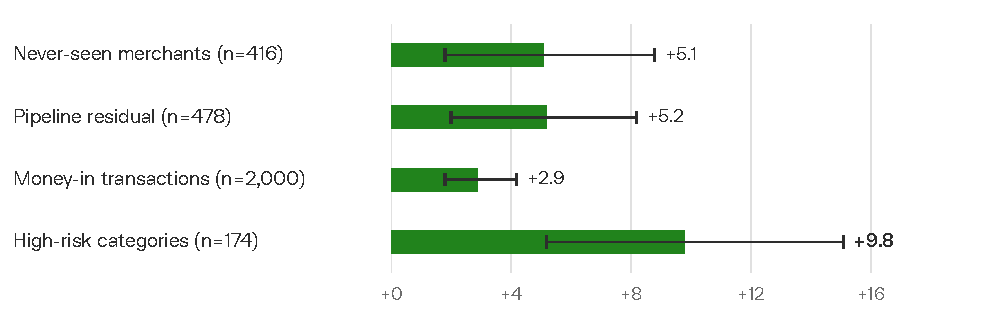
\includegraphics[width=\linewidth]{charts/fig-transformer.pdf}
\caption*{Leaf-level accuracy, mean of three seeds, paired bootstrap on the same rows. Every interval sits above zero. General-level gains are larger still, at 7 to 13 points.}
\end{figure}
Every accuracy criterion set at the start now clears with confidence intervals excluding zero. The remaining cost is speed: the transformer scores at about a third of the linear model's rate, which is roughly 70 CPU-minutes for the full Plaid table and has been judged acceptable for now. Quantisation would recover a factor of two to three if it becomes a constraint.

It is worth being clear about what the transformer did and did not do. The full-pipeline number moved by one point, because 76\% of transactions never reach the classifier. Its value is concentrated where the rules cannot help: on merchants nobody has labelled, and on the high-risk categories that the credit model cares about most.

